
\subsection{Faraday-Effekt}
\begin{figure}[h]
\begin{center}
\includegraphics[scale=0.3]{auf_fara}
\caption{Versuchsaufbau zum Faraday-Effekt; (1)Wasserkühlung, (2)Spule mit Schwerflintstab, (3)Na-Lampe, (4)Analysator des Halbschattenpolarimeters, (5)Okular; Quelle: [ver]}
\label{fig:auf_fara}
\end{center}
\end{figure}
\begin{floatingfigure}[l]{8.0cm}
\begin{center}
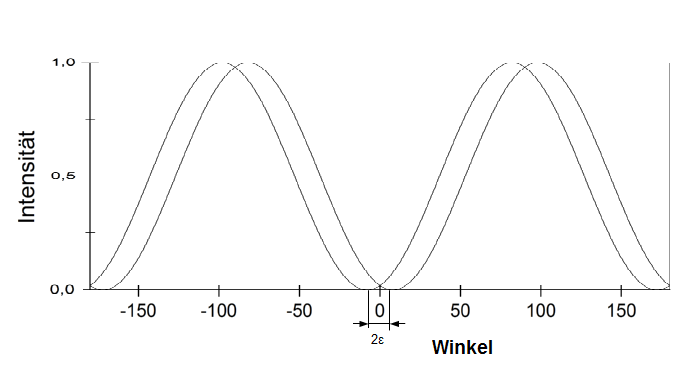
\includegraphics[scale=0.27]{2epsilon2}
\caption{Theoretische Intensität der beiden vom Halbschattenpolarimeter erzeugten Flächen.}
\label{fig:2epsilon}
\end{center}
\end{floatingfigure}
 Der Aufbau ist wie in Abbildung \ref{fig:auf_fara} gegenben. Einige Minuten vor Beginn der Versuchsdurchführung wird die Wasserkühlen der Spule und die Natriumdampflampe angeschaltet. Um später den Ablesefehler besser abschätzen zu können wurden hier zu beginn mehrere Messwerte aufgenommen für den Ablenkwinkel bei einem Spulenstrom von $I=0A$. Dabei das Halbschattenpolarimeter mehrmals von der Ausgleichslage (Position bei der die Felder gleich hell sind) weg gedreht und frisch eingestellt.
Nun wurden die Winkel für verschieden Stromstärken gemessen, es wird in $0,5A$ Schritten von etwa $-4,5A$ bis $+4,5A$ gemessen. Dabei wird der Winkel in der Ausgleichslage zur jeweiligen Stromstärke notiert.\\
Um den $2 \epsilon$-Winkel, der Winkel um welchen die Hälften zueinander verschoben sind,zu bestimmen, muss einmal der Winkel gemessen werden bei dem die (hier) äußeren Flächen am dunkelsten sind und die innere Fläche am hellsten und den Winkel bei der inversen Helligkeitsauflösung. Der $2 \epsilon$-Winkel ist dabei die Differenz der beiden gemessenen Winkel.
